%*****************************************
\chapter{Evaluation}
\label{ch:evaluation}
%*****************************************
%\hint{This chapter should describe how the evaluation of the implemented mechanism was done. \\ \\
%1. Which evaluation method is used and why? Simulations, prototype? \\
%2. What is the goal of the evaluation? Comparison? Proof of concept? \\
%3. Wich metrics are used for characterizing the performance, costs, fairness, and efficiency of the system?\\
%4. What are the parameter settings used in the evaluation and why? If possible always justify why a certain threshold has been chose for a particular parameter.  \\
%5. What is the outcome of the evaluation? \\ \\
%The section should have a length of about five to ten pages.}
The following chapter presents the results achieved throughout this thesis and aims to explain their evaluation. First, the intended goal of each experiment is stated, including a  formulation in terms of validatable benchmarks. Subsequently, the process which extracts legible data from the framework is developed. The visualized data follows, and finally, the results are analyzed.

\section{Goal and Benchmarks}
\subsection*{Reproduction}
As the latter sections evaluate explorative experiments, the validity of the framework which supports them is crucial. The first two models described in sections [4] and [5] were trained under the exact conditions J. Frankle and M. Corbin describe in their paper. The mismatch of weights previously described forms the only difference.
J. Frankle and M. Corbin report three different measures of their experiments: the test accuracy during training, the iteration of a primary early stopping criterion, and the accuracy at the early stopping criterion. As shown in [Figure], they displayed all these criteria with margins of confidence obtained by averaging five experiments. The goal of this reproduction is to produce results within the reported confidence intervals.  
\subsection*{Early Tickets}
The third experiment aims to establish whether the Lottery Ticket Hypothesis holds in the context of similar tasks on datasets of other fields. While J. Frankle and M. Carbin define a lottery ticket as any pruned network that achieves better training results than its complete counterpart [cite], lottery tickets bigger than partial networks discovered by contemporary pruning algorithms would be of little value. The related works in chapter [3] present pruning rates of about 90 percent. A lottery ticket search reaches this magnitude of reduction in ten pruning iterations. If, at that point, the quality of the remains at least the same, the proof-of-concept is valid.
\subsection*{Transfer}
As J. Frankle and M. Carbin do not deal with the question of whether complete training is necessary to obtain lottery tickets, the last experiment of this thesis intends to establish a proof-of-concept for early lottery ticket retrieval. For the same reasons as before the requirements for a valid lottery ticket are: 
A pruning rate of about 90 or above and consistent quality of the network.

\section{Evaluation Setup}
\subsection*{Reproduction}
Because of the difficulties between framework and backend, chapter 5 describes, no early stopping criterion is available. Furthermore, each of the results of multiple runs of the same experiment were identical, which invalidates the use of confidence intervals. A practical solution is to display the full range of accuracies from the point the network starts to converge. Additionally, this setup benefits the following explorative experiments because it is parameter-agnostic towards the early stopping criterion. Finally, for the MNIST-Lenet-FCN architecture, the accuracies during training remain for comparison.
\subsection*{Transfer}
In the sake of consistency, the presented values are of the same kind as in the first experiment. Additional visualization is available in [appendix A].
\subsection*{Early Tickets}




\section{Evaluation Results}
\subsection*{Reproduction}
\begin{figure}
	\begin{minipage}{0.5\textwidth}
		\centering
		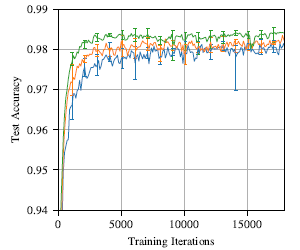
\includegraphics[height=175px]{gfx/7-Evaluation/LTH_1.png}
		\caption*{LTH-paper: Lenet-FCN 0|3|7}
		\label{?}
	\end{minipage}\hfill
	\begin{minipage}{0.5\textwidth}
		\centering
		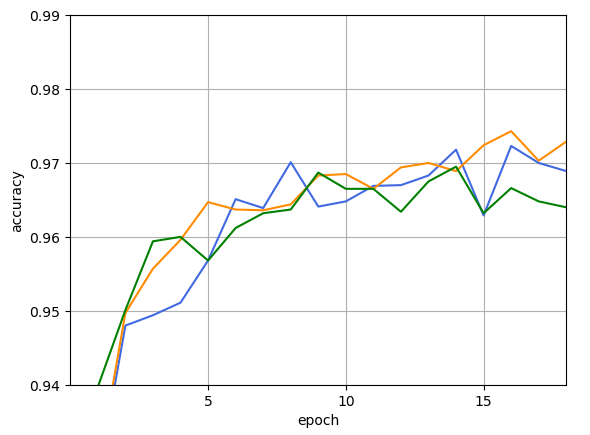
\includegraphics[height=175px]{gfx/Experiments/Reproduction-MNIST-FCN/accuracy/LTH_1.png}
		\caption*{Thesis-Framework: Lenet-FCN 0|3|7}
		\label{?}
	\end{minipage}
	\\[10pt]
	\begin{minipage}{0.5\textwidth}
		\centering
		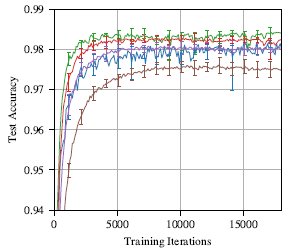
\includegraphics[height=175px]{gfx/7-Evaluation/LTH_2.png}
		\caption*{LTH-paper: Lenet-FCN 0|7|12|15|18}
		\label{?}
	\end{minipage}\hfill
	\begin{minipage}{0.5\textwidth}
		\centering
		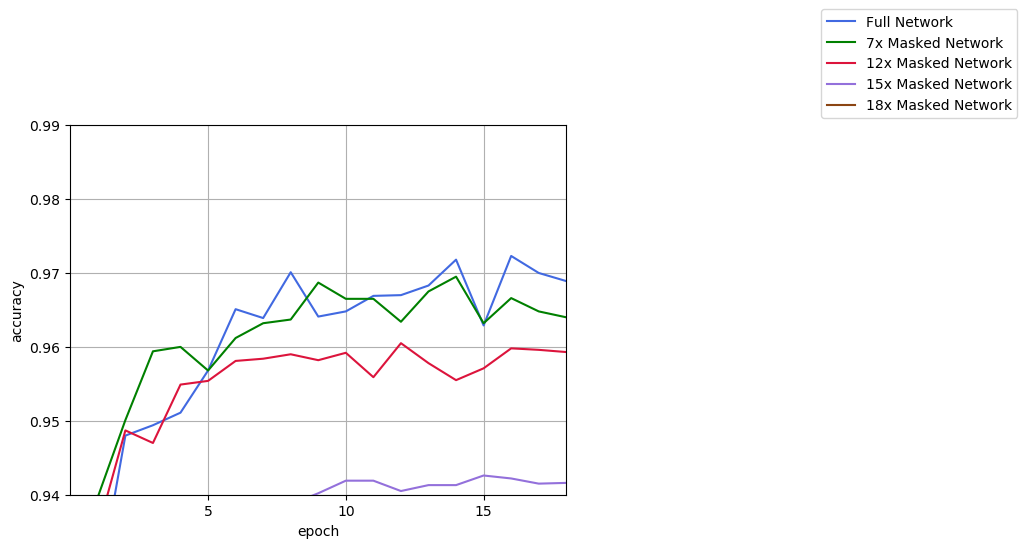
\includegraphics[height=175px]{gfx/Experiments/Reproduction-MNIST-FCN/accuracy/LTH_2.png}
		\caption*{Thesis-Framework: Lenet-FCN 0|7|12|15|18}
		\label{?}
	\end{minipage}
	\\
	\begin{minipage}{0.5\textwidth}
		\centering
		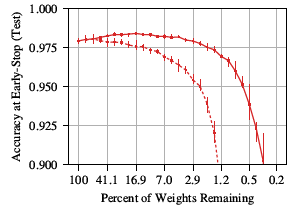
\includegraphics[height=175px]{gfx/7-Evaluation/LTH_0.png}
		\caption*{LTH-paper: Accuracy after convergence\\
			(random w. | initial w.)}
		\label{?}
	\end{minipage}\hfill
	\begin{minipage}{0.5\textwidth}
		\centering
		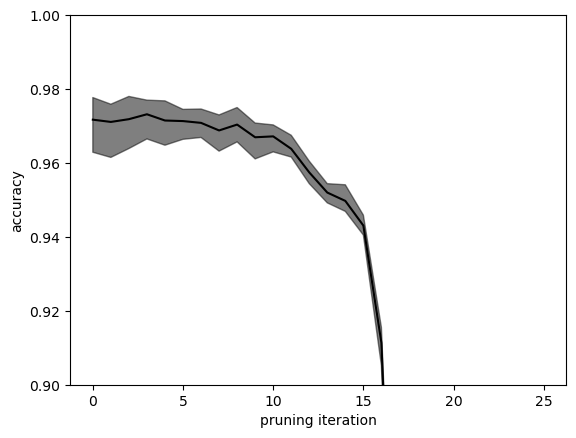
\includegraphics[height=175px]{gfx/Experiments/Reproduction-MNIST-FCN/accuracy/converged.png}
		\caption*{Thesis-Framework: Accuracy after convergence}
		\label{?}
	\end{minipage}
\end{figure}
\begin{figure}
	\begin{minipage}{0.5\textwidth}
		\centering
		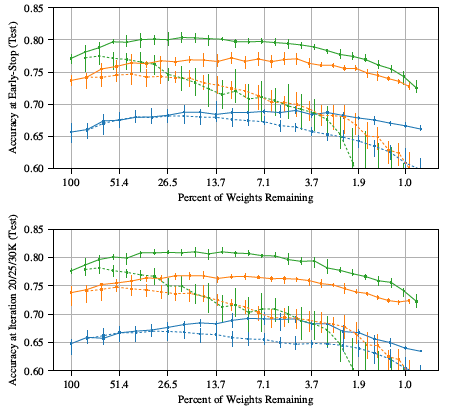
\includegraphics[height=175px]{gfx/7-Evaluation/LTH_CNN.png}
		\caption*{Accuracy on CIFAR10 over 10 pruning iterations}
		\label{fig:CIFAR10accuracy10}
	\end{minipage}\hfill
	\begin{minipage}{0.5\textwidth}
		\centering
		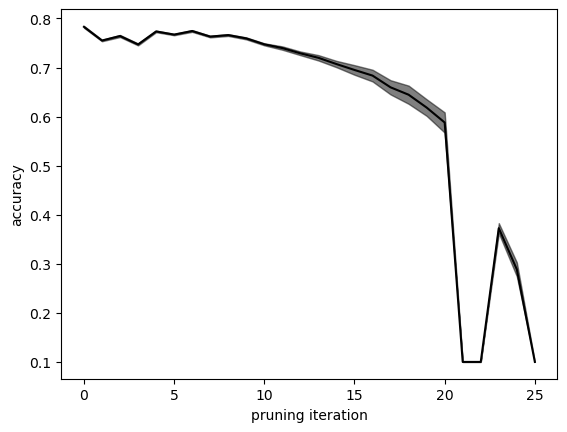
\includegraphics[height=175px]{gfx/Experiments/Reproduction-CIFAR10-CNN/accuracy/converged.png}
		\caption*{Accuracy on CIFAR10 over 15 pruning iterations}
		\label{fig:CIFAR10accuracy15}
	\end{minipage}
\end{figure}
\subsection*{Early Tickets}
\subsection*{Transfer}
\begin{figure}
	\begin{minipage}{0.5\textwidth}
		\centering
		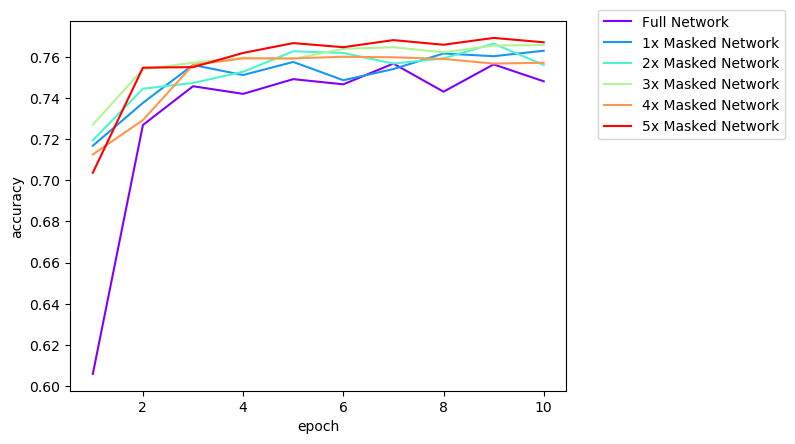
\includegraphics[width=220px]{gfx/Experiments/Transfer-20Newsgroups-CNN/accuracy/5_iterations.png}
		\caption*{Accuracy on 20Newsgroups over 5 pruning iterations}
		\label{fig:CIFAR10accuracy10}
	\end{minipage}\hfill
	\begin{minipage}{0.5\textwidth}
		\centering
		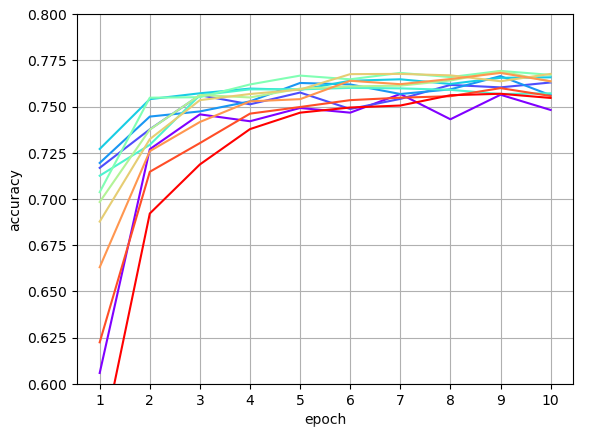
\includegraphics[width=220px]{gfx/Experiments/Transfer-20Newsgroups-CNN/accuracy/10_iterations.png}
		\caption*{Accuracy on 20Newsgroups over 10 pruning iterations}
		\label{fig:CIFAR10accuracy15}
	\end{minipage}
\end{figure}

\section{Analysis of Results}
\subsection*{Reproduction}
\subsection*{Early Tickets}
\subsection*{Transfer}
